\subsection{Hahn Echo} \label{B5}

\begin{comment}
\begin{itemize}
\item talk about what the hahn echo is and how we're measuring it \textbf{(10 mins)}
\item Show how you found the magnetization data points for one of the samples ****this involves probably shifting the graphs up so that they approach 0****  (show a plot with a labeled data point) \textbf{(10 min)}
\item find the magnetization data points for each of the graphs and uncertainties \textbf{(15 mins)}
\item plot the values obtained for each of the samples, include a graph with error bars (the uncertainties from above), there should be horiziontial and vertical bars because we're approximating both the time and voltage. given units and a title. \textbf{(15 mins)}
\item fit an exp to each plot and say which function and language you're using \textbf{(15 mins)}
\item say the coefficients of the each fit and the uncertainties \textbf{(10 mins)}
\item show a sample calculation for $T_2$ and its uncertainty \textbf{(10 mins)}
\item talk about each of the fits, causes for errors etc. and the physics for why the $T_2$'s may be different \textbf{(15 mins)}
\end{itemize}
\end{comment}




The raw data collected from the spectrometer was zero-shifted and smoothed using a simple Gaussian filtering procedure (see Appendix \ref{append:process}). The peak magnetization of the echo decays as,
\begin{align*}
    M(t) &= M_0 e^{-t/T_2}\\
    \intertext{Similar to previous sections, taking the natural logarithm and rearranging,}
    \ln \left( M(t) \right) &= \frac{-t}{T_2} + \ln(M_0) \numberthis \label{eqn:B5:log}
\end{align*}

Figure \ref{fig:B5:fit/trace} shows each trace with different time-delays and the calculated echo amplitude. These amplitudes are plotted against $t=2\tau$ in Figure \ref{fig:B5:expcurve}, along with the fit -- which was determined using a linear least squares regression of the data, using the form from Equation \ref{eqn:B5:log}. From the fit, the $T_2$ value is the slope of the line, and the uncertainty is the 95\% confidence interval of the least squares algorithm. The $T_2$ values for doped water, ethanol and rubber are summarized in Table \ref{tab:B5:T2vals}.

\begin{figure}[H]
    \centering
    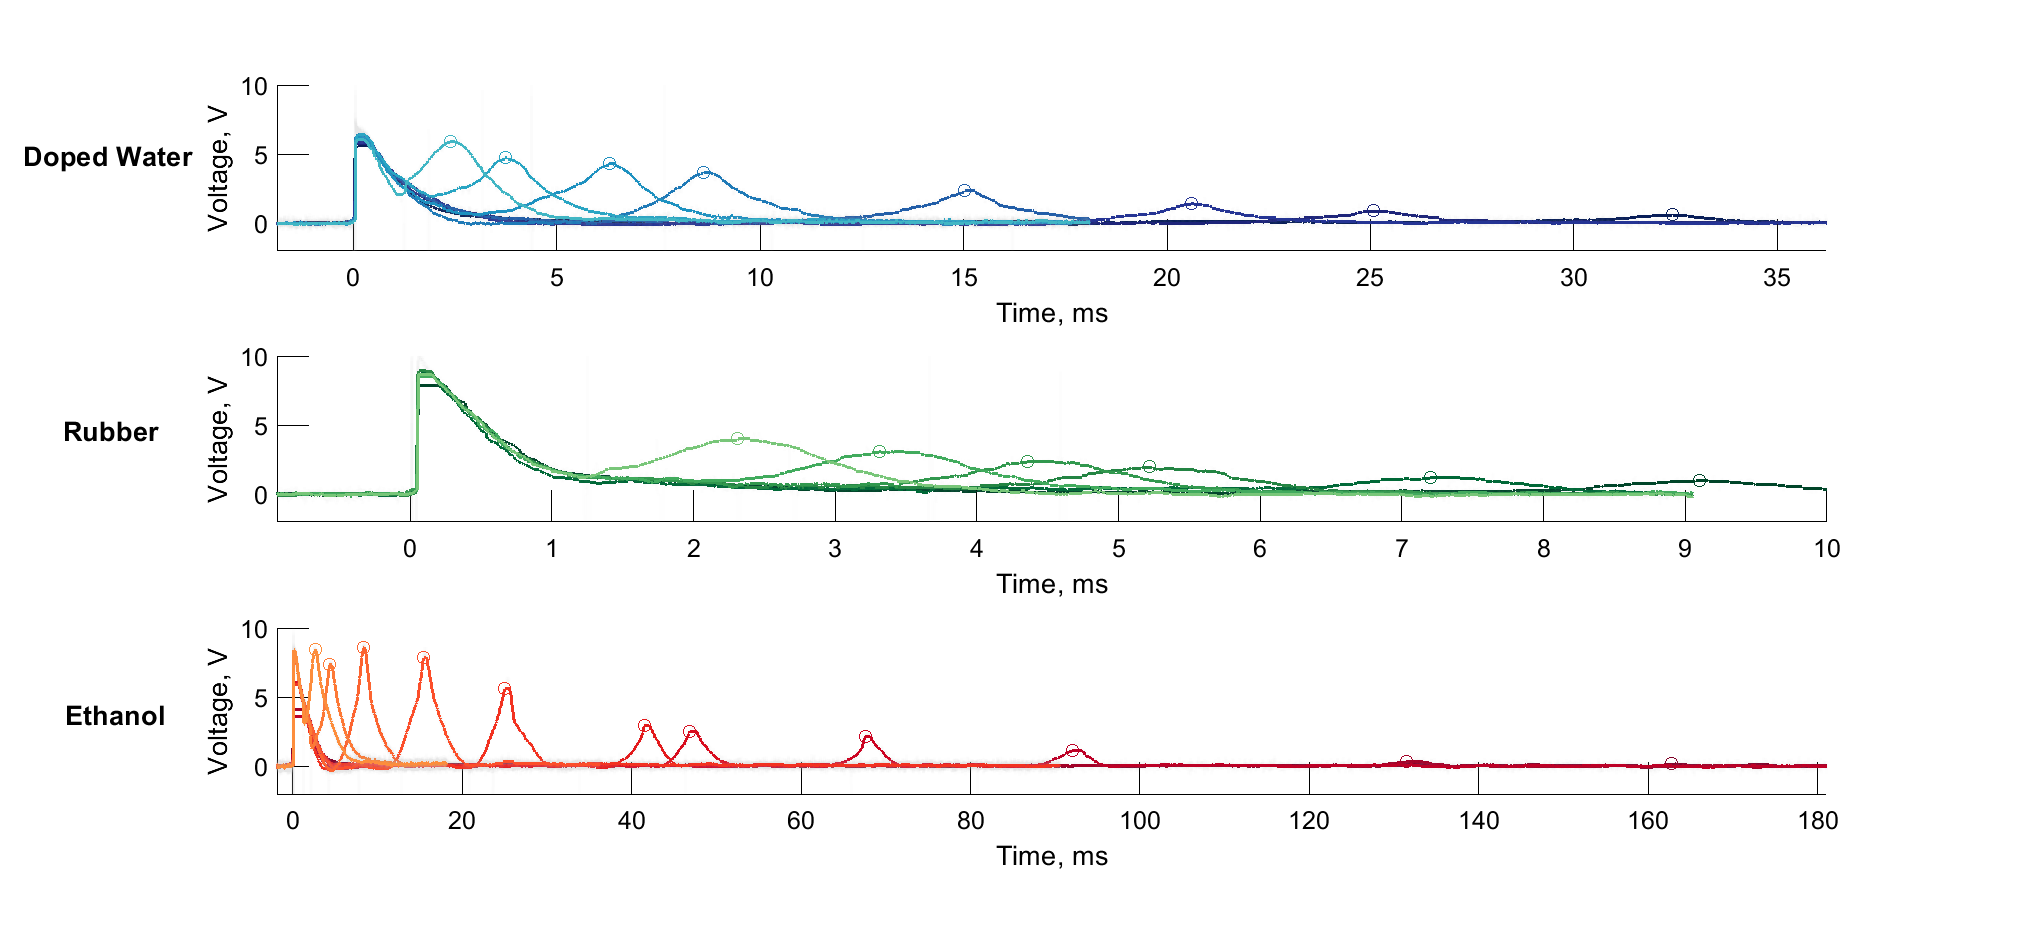
\includegraphics[width=\textwidth]{figures/B5/B5_1.eps}
    \caption{Time traces of Hahn echo experiments for the samples, with multiple traces for time-delay $\tau$ overlaid. The solid lines are the filtered data, light grey is the raw, unfiltered data, and the circle points are the calculated peak magnetization values at $t=2\tau$.}
    \label{fig:B5:fit/trace}
\end{figure}

\begin{figure}[H]
    \centering
    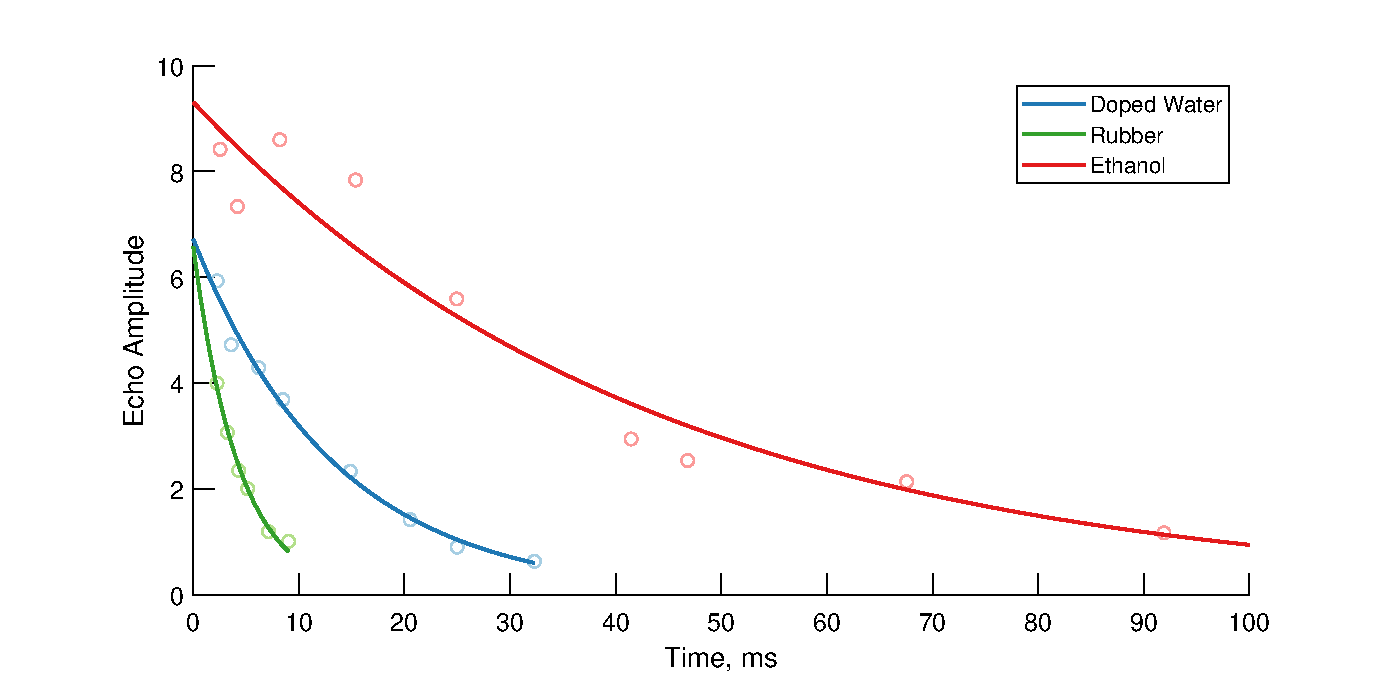
\includegraphics[width=\textwidth]{figures/B5/B5_2.eps}
    \caption{Peak magnetization of three samples, extracted from Figure \ref{fig:B5:fit/trace} to determine $T_2$.}
    \label{fig:B5:expcurve}
\end{figure}

\begin{table}[H]
    \centering
    \begin{tabular}{c|c}
    \toprule
    \textbf{Sample} & $T_2$ (ms) \\ \midrule
        Doped Water &  $13.31 \pm 1.16$ \\
        Ethanol &  $42.21 \pm 3.38$ \\
        Rubber &  $4.80 \pm 1.11$ \\ \bottomrule
    \end{tabular}
    \caption{$T_2$ values for three samples determined using the Hahn echo experiments, calculated from the fit of results from Figure \ref{fig:B5:expcurve}.}
    \label{tab:B5:T2vals}
\end{table}

As expected from Equation \ref{eqn:Hanecho}, 
\[ 1/T^*_2 = 1/T_2 + \gamma \Delta B_o \]
all values of $T_2$ are greater than that of $T_2^*$ (Table \ref{tab:B2:T2*_values}). Using these two terms, it is straightforward to calculate the $\gamma\Delta B_o$ values for each sample. As $\gamma$ is constant for each sample (the gyromagnetic ratio of a proton) then from Table \ref{tab:B5:hom} we can compare the relative field inhomogeneities of each sample. We can see that rubber has greater field inhomogeneities than the liquid sample ethanol by a factor of approximately two. The rubber sample used here, a pencil eraser, likely has manufacturing impurities and spatial differences in density and chemical composition -- compared to a highly pure sample of ethanol. Thus, it is consistent with our knowledge of the samples that the field inhomogeneities of rubber are greater than the other two samples. 
\begin{table}[H]
    \centering
    \begin{tabular}{c|c} \toprule
        \textbf{Sample} & $\gamma \Delta B_o$ (ms$^{-1}$) \\ \midrule
        Doped Water & $0.7876\pm0.0126$ \\
        Ethanol & $1.0816\pm0.0100$ \\
        Rubber & $2.1987\pm0.0362$ \\ \bottomrule
    \end{tabular}
    \caption{Comparison of the field inhomogeneities for each sample, computed from the differences in $T_2$ (Section \ref{B4}, IR method) and $T_2^*$ (Section \ref{B2}).}
    \label{tab:B5:hom}
\end{table}